% =============================================================
% Tutorial paso a paso del algoritmo del Capítulo 2:
% Construcción de la intersección de una PRCG con un lenguaje regular
% =============================================================
% Este documento es interno: sirve para entender el algoritmo antes de
% redactar el capítulo. No es parte de la tesis.
% =============================================================

\documentclass[11pt, letterpaper]{article}

% --- Codificación e idioma ---
\usepackage[utf8]{inputenc}
\usepackage[T1]{fontenc}
\usepackage[spanish, provide=*]{babel}

% --- Matemáticas ---
\usepackage{amsmath}
\usepackage{amssymb}
\usepackage{amsthm}
\usepackage{mathtools}

% --- Layout ---
\usepackage[margin=1in]{geometry}
\usepackage{parskip}
\setlength{\parindent}{0pt}
\setlength{\parskip}{0.7ex plus 0.2ex minus 0.1ex}

% --- Tipografía y enlaces ---
\usepackage{microtype}
\usepackage[hidelinks]{hyperref}
\usepackage{xcolor}

% --- Diagramas (autómatas) ---
\usepackage{tikz}
\usetikzlibrary{automata, positioning, arrows.meta, calc}

% --- Pseudocódigo ---
\usepackage{algorithm}
\usepackage{algpseudocode}
\algrenewcommand\algorithmicrequire{\textbf{Entrada:}}
\algrenewcommand\algorithmicensure{\textbf{Salida:}}
\floatname{algorithm}{Algoritmo}

% --- Bloques de código ---
\usepackage{fancyvrb}

% --- Cajas de resaltado ---
\usepackage{tcolorbox}
\tcbset{colback=blue!5!white, colframe=blue!50!black, boxrule=0.5pt,
        arc=2pt, left=4pt, right=4pt, top=3pt, bottom=3pt}

% --- Entornos ---
\theoremstyle{definition}
\newtheorem{ejemplo}{Ejemplo}
\newtheorem{paso}{Paso}

% --- Macros ---
\newcommand{\PRCG}{\mbox{PRCG}}
\newcommand{\AFD}{\mbox{AFD}}
\newcommand{\sRCG}{\mbox{sRCG}}
\newcommand{\eps}{\varepsilon}
\newcommand{\pair}[2]{\langle #1, #2 \rangle}
\newcommand{\trans}{\delta}
\newcommand{\transit}{\delta^{*}}
\newcommand{\hl}[1]{\textcolor{red!70!black}{\textbf{#1}}}
\newcommand{\Par}{\mathrm{Par}}

\renewcommand{\proofname}{Demostración}

\title{\textbf{Tutorial paso a paso del algoritmo de intersección \PRCG\ $\cap$ regular} \\[0.4em]
\large Una guía visual con un ejemplo trabajado completo}
\author{}
\date{}

\begin{document}
\maketitle
\thispagestyle{empty}

\begin{tcolorbox}
\textbf{Propósito de este documento.} El Capítulo 2 de la tesis define un algoritmo que, dada una \PRCG\ $G$ y un autómata finito determinista $A$, construye una nueva \PRCG\ $G'$ tal que $L(G') = L(G) \cap L(A)$. Este documento presenta el algoritmo paso a paso sobre un ejemplo concreto, desarrollando todas las cláusulas y trazando una derivación completa al final.
\end{tcolorbox}

% =============================================================
\section{El problema en una frase}

Se parte de una \PRCG\ $G$ que genera un lenguaje $L(G)$, y un \AFD\ $A$ que reconoce un lenguaje regular $L(A)$. Se desea construir una \PRCG\ $G'$ tal que el lenguaje que genera $G'$ sea exactamente $L(G) \cap L(A)$, esto es, las cadenas que pertenecen a ambos lenguajes simultáneamente.

\begin{tcolorbox}
\textbf{Idea fundamental.} En lugar de razonar sobre rangos $\langle i, j \rangle$ que apuntan a posiciones de una cadena fija $w$, la construcción razona sobre \emph{pares de estados} $\langle p, p' \rangle$ del autómata $A$. Un par $\langle p, p' \rangle$ representa una subcadena que lleva $A$ del estado $p$ al estado $p'$.
\end{tcolorbox}

% =============================================================
\section{Hipótesis sobre la \PRCG\ de entrada}

El algoritmo del presente tutorial trata las \PRCG\ \emph{top-down non-erasing}, en el sentido de Boullier~\cite{REF}: una \PRCG\ $G$ es top-down non-erasing si, para toda cláusula $c$ de $G$, cada variable que aparece en la cabeza de $c$ aparece también en el cuerpo de $c$. La restricción es sintáctica y se verifica por inspección directa de las cláusulas.

La restricción no es una limitación esencial. Por la cadena de Properties~1, 2 y 3 de Boullier~\cite{REF}, toda \PRCG\ admite una versión equivalente que es no-combinatorial y non-erasing, la cual es en particular top-down non-erasing. La transformación que produce la versión equivalente queda fuera del alcance del tutorial: la gramática que sirve de entrada al algoritmo se asume top-down non-erasing.

La clase top-down non-erasing es estrictamente más amplia que la clase \sRCG\ tratada por Bertsch y Nederhof~\cite{REF}: admite cláusulas no-lineales, como las del ejemplo motivador que se desarrolla en la sección siguiente, y cláusulas combinatorias, en las que un argumento del cuerpo contiene terminales mezclados con variables.

% =============================================================
\section{Ejemplo de partida}

% --- La gramática G ---
\subsection{La gramática $G$}

Sea $G = (N, T, V, P, S)$ con $N = \{S, \Par\}$, $T = \{a\}$, $V = \{X\}$, axioma $S$, y las cláusulas siguientes:

\begin{tcolorbox}[colback=yellow!10, colframe=orange!60!black]
\begin{align*}
c_1: &\quad S(X)        \to \Par(X) \; \Par(X) \\
c_2: &\quad \Par(aaX)    \to \Par(X) \\
c_3: &\quad \Par(\eps)   \to \eps
\end{align*}
\end{tcolorbox}

\textbf{Qué genera esta gramática.} Cada cláusula tiene un rol específico:

\begin{itemize}
\item $c_1$: el predicado $S$ deriva una cadena $X$ que pasa simultáneamente por dos invocaciones de $\Par$. La variable $X$ aparece tres veces en la cláusula: una en la cabeza y dos en el cuerpo. La semántica de \PRCG\ exige que las tres ocurrencias representen la misma cadena.
\item $c_2$: $\Par$ aplicada a una cadena que empieza con $aa$ se reduce a $\Par$ aplicada al resto.
\item $c_3$: $\Par$ acepta la cadena vacía.
\end{itemize}

Las cláusulas $c_2$ y $c_3$ definen $\Par$ como el conjunto de cadenas sobre $\{a\}$ con longitud par, esto es, $\{a^{2n} : n \geq 0\}$. La cláusula $c_1$ exige que la cadena entera sea aceptada por $\Par$ de manera simultánea por las dos invocaciones que deben coincidir. Por tanto $L(G) = \{a^{2n} : n \geq 0\}$.

\textbf{No-linealidad top-down.} La variable $X$ aparece dos veces en el cuerpo, una vez en cada $\Par$. Esto rompe la condición de \emph{linealidad top-down} de Boullier~\cite{REF}, Definición~8: ninguna variable puede aparecer más de una vez en la unión de los argumentos del cuerpo. La cláusula $c_1$ es \hl{no-lineal top-down}, y la situación en la que la condición \textbf{C2} de la construcción actúa de manera no trivial.

\textbf{Top-down non-erasing.} La gramática $G_0$ cumple la hipótesis del tutorial: en cada cláusula, toda variable de la cabeza aparece también en el cuerpo. En $c_1$, la variable $X$ aparece en la cabeza y en los dos predicados del cuerpo. En $c_2$, la variable $X$ aparece en la cabeza y en el único predicado del cuerpo. En $c_3$, no hay variables. La hipótesis se cumple por tanto en las tres cláusulas.

% --- El autómata A ---
\subsection{El autómata $A$}

Sea $A = (Q, T, \trans, q_0, F)$ con $Q = \{q_0, q_1, q_2\}$, $T = \{a\}$, estado inicial $q_0$ y estados finales $F = \{q_0\}$. Las transiciones son
\[
\trans(q_0, a) = q_1, \qquad \trans(q_1, a) = q_2, \qquad \trans(q_2, a) = q_0.
\]

El autómata se representa gráficamente como sigue.

\begin{center}
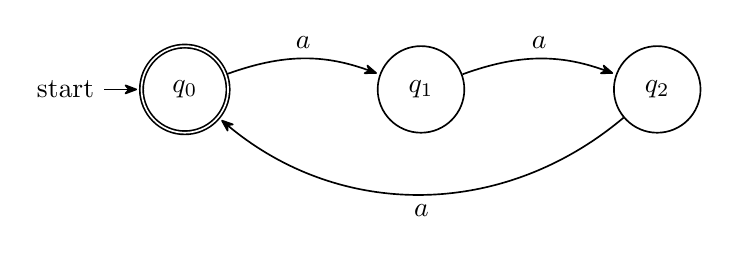
\begin{tikzpicture}[->, >={Stealth[round]}, shorten >=1pt, auto, node distance=3cm, semithick, every state/.style={minimum size=1.1cm}]
  \node[state, initial, accepting]   (q0)              {$q_0$};
  \node[state]                       (q1) [right of=q0] {$q_1$};
  \node[state]                       (q2) [right of=q1] {$q_2$};

  \path
    (q0) edge [bend left=20]  node {$a$} (q1)
    (q1) edge [bend left=20]  node {$a$} (q2)
    (q2) edge [bend left=40]  node [below] {$a$} (q0);
\end{tikzpicture}
\end{center}

El autómata $A$ acepta una cadena si y solo si su longitud es múltiplo de 3:
\[
L(A) = \{ a^{3k} : k \geq 0 \} = \{\eps, aaa, aaaaaa, a^9, a^{12}, \ldots\}.
\]

% --- La intersección ---
\subsection{La intersección por construir}

Una cadena pertenece a $L(G) \cap L(A)$ si y solo si pertenece a ambos lenguajes:
\[
L(G) \cap L(A) = \{ a^{2n} : n \geq 0 \} \cap \{ a^{3k} : k \geq 0 \} = \{ a^{6m} : m \geq 0 \}.
\]

El conjunto resultante son las cadenas de $a$ con longitud múltiplo de 6: $\{\eps, aaaaaa, a^{12}, a^{18}, \ldots\}$.

% =============================================================
\section{La idea de la construcción}

\begin{tcolorbox}
Cada predicado $B$ de $G$ con aridad $k$ se reemplaza por una colección de versiones indexadas $B[\vec{q}]$, donde $\vec{q}$ es un vector con $k$ pares de estados, uno por cada argumento de $B$.

\smallskip
\textbf{El predicado $B[\pair{p}{p'}]$ aplicado al rango $\pair{i}{j}$ deriva exactamente cuando:}
\begin{itemize}
\item el predicado $B$ original aplicado al mismo rango deriva en $G$, \emph{y}
\item el autómata $A$ leyendo la subcadena $w[i+1 \ldots j]$ va de $p$ a $p'$.
\end{itemize}
\end{tcolorbox}

% =============================================================
\section{Construcción de $G'$ paso a paso}

% --- Paso 1: no terminales ---
\begin{paso}[Crear los predicados indexados]
\end{paso}

El conjunto $N'$ de no terminales de $G'$ se construye así:

\begin{itemize}
\item Un nuevo símbolo distinguido $S'$ de aridad 1.
\item Por cada predicado $B \in N$ de aridad $k$ y cada vector $\vec{q} \in (Q \times Q)^k$, un nuevo símbolo $B[\vec{q}]$ de aridad $k$.
\end{itemize}

En el ejemplo, $S$ y $\Par$ tienen aridad 1, así que cada uno produce $|Q|^{2} = 9$ versiones indexadas. El total es $1 + 9 + 9 = 19$ símbolos no terminales.

% --- Paso 2: cláusulas iniciales ---
\begin{paso}[Cláusulas iniciales: conectar $S'$ con $S$ indexada]
\end{paso}

Por cada estado final $q \in F$ se añade una cláusula
\[
S'(X) \to S[\pair{q_0}{q}](X).
\]

Esta cláusula expresa que $S'$ acepta $X$ siempre que $S$ leyendo $X$ vaya del estado inicial $q_0$ a algún estado final $q$. Esa es la condición precisa para que $X$ sea aceptada por el autómata $A$.

En el ejemplo, $F = \{q_0\}$, así que solo se añade una cláusula inicial:

\begin{tcolorbox}[colback=green!10, colframe=green!50!black]
\textbf{Cláusula inicial:} $\quad S'(X) \to S[\pair{q_0}{q_0}](X)$
\end{tcolorbox}

% --- Paso 3: cláusulas heredadas de c1 ---
\begin{paso}[Cláusulas heredadas de $c_1$ --- donde \textbf{C2} actúa]
\end{paso}

La cláusula original es $c_1: S(X) \to \Par(X) \; \Par(X)$. La construcción genera todas las instancias indexadas que satisfagan las condiciones \textbf{C1} y \textbf{C2}.

\begin{itemize}
\item \textbf{C1 (coherencia interna):} en cada argumento de la cláusula, las transiciones del autómata sobre los terminales y los pares asignados a las variables deben encajar.
\item \textbf{C2 (coherencia entre ocurrencias):} si una variable $X$ aparece varias veces en la cláusula, todas sus ocurrencias deben llevar el mismo par de estados.
\end{itemize}

La variable $X$ aparece tres veces en $c_1$: una en la cabeza y dos en los predicados $\Par$ del cuerpo. Por \textbf{C2}, las tres ocurrencias deben tener el \hl{mismo} par de estados. Sea $\Phi(X) = \pair{p}{p'}$ ese par único.

Aplicando \textbf{C1} al argumento de la cabeza, que consta únicamente de la variable $X$, el par del argumento de la cabeza coincide directamente con $\pair{p}{p'}$. Lo mismo vale para los argumentos de los dos $\Par$ en el cuerpo: ambos llevan el par $\pair{p}{p'}$.

La cláusula instanciada es
\[
S[\pair{p}{p'}](X) \to \Par[\pair{p}{p'}](X) \; \Par[\pair{p}{p'}](X).
\]

Como $\Phi(X)$ recorre los 9 pares posibles, se generan 9 cláusulas heredadas a partir de $c_1$. La cláusula alcanzable desde la cláusula inicial $S'(X) \to S[\pair{q_0}{q_0}](X)$ es

\begin{tcolorbox}[colback=green!10, colframe=green!50!black]
\textbf{Heredada alcanzable de $c_1$:}
\[
S[\pair{q_0}{q_0}](X) \to \Par[\pair{q_0}{q_0}](X) \; \Par[\pair{q_0}{q_0}](X)
\]
\end{tcolorbox}

\begin{tcolorbox}
\textbf{Consecuencia de omitir \textbf{C2}.} Sin \textbf{C2}, las tres ocurrencias de $X$ podrían recibir pares distintos. Por ejemplo, una cláusula heredada que viola \textbf{C2} sería
\[
S[\pair{q_0}{q_0}](X) \to \Par[\pair{q_0}{q_1}](X) \; \Par[\pair{q_1}{q_0}](X),
\]
en la que la misma $X$ tendría que ser una cadena que vaya simultáneamente de $q_0$ a $q_1$ y de $q_1$ a $q_0$, situación imposible para una sola subcadena. La verificación operacional reportada en el Capítulo~2 confirma que sin \textbf{C2}, la gramática producto sobre-genera con cadenas como $aa$ y $aaaa$, que pertenecen a $L(G)$ pero no a $L(A)$.
\end{tcolorbox}

% --- Paso 4: cláusulas heredadas de c2 ---
\begin{paso}[Cláusulas heredadas de $c_2$ --- consumo de terminales]
\end{paso}

La cláusula original es $c_2: \Par(aaX) \to \Par(X)$. La variable $X$ tiene dos ocurrencias, una en la cabeza dentro del argumento $aaX$ y otra en el cuerpo. Por \textbf{C2}, ambas reciben el mismo par $\Phi(X) = \pair{p}{p'}$.

\textbf{C1} aplicada al argumento de la cabeza, $\alpha = aaX$, descompuesto como $\beta_1 = a$, $\beta_2 = a$, $\beta_3 = X$, exige una sucesión de estados $r_0 = p_0$, $r_1$, $r_2$, $r_3 = p'_0$ tal que
\begin{itemize}
\item $\beta_1 = a$ implica $\trans(r_0, a) = r_1$,
\item $\beta_2 = a$ implica $\trans(r_1, a) = r_2$,
\item $\beta_3 = X$ implica $\pair{r_2}{r_3} = \pair{p}{p'}$, esto es $r_2 = p$ y $r_3 = p'$.
\end{itemize}

Combinando las tres condiciones, $\trans(\trans(p_0, a), a) = p$. El estado $p_0$ es el predecesor de $p$ por dos transiciones de $a$. En el autómata $A$, dos transiciones de $a$ corresponden a un avance de dos estados, que se condensa en la siguiente tabla.

\begin{center}
\begin{tabular}{c|c}
$p$ & $\text{pred}^2(p) = p_0$ tal que $\trans^2(p_0, aa) = p$ \\
\hline
$q_0$ & $q_1$ \\
$q_1$ & $q_2$ \\
$q_2$ & $q_0$
\end{tabular}
\end{center}

Para cada elección de $\Phi(X) = \pair{p}{p'}$, con $9$ opciones, la cláusula instanciada es
\[
\Par[\pair{\text{pred}^2(p)}{p'}](aaX) \to \Par[\pair{p}{p'}](X).
\]

Las 9 cláusulas heredadas de $c_2$ se enumeran a continuación.

\begin{tcolorbox}[colback=green!10, colframe=green!50!black]
\textbf{Heredadas de $c_2$:}
\begin{align*}
& \Par[\pair{q_1}{q_0}](aaX) \to \Par[\pair{q_0}{q_0}](X) \\
& \Par[\pair{q_1}{q_1}](aaX) \to \Par[\pair{q_0}{q_1}](X) \\
& \Par[\pair{q_1}{q_2}](aaX) \to \Par[\pair{q_0}{q_2}](X) \\
& \Par[\pair{q_2}{q_0}](aaX) \to \Par[\pair{q_1}{q_0}](X) \\
& \Par[\pair{q_2}{q_1}](aaX) \to \Par[\pair{q_1}{q_1}](X) \\
& \Par[\pair{q_2}{q_2}](aaX) \to \Par[\pair{q_1}{q_2}](X) \\
& \Par[\pair{q_0}{q_0}](aaX) \to \Par[\pair{q_2}{q_0}](X) \\
& \Par[\pair{q_0}{q_1}](aaX) \to \Par[\pair{q_2}{q_1}](X) \\
& \Par[\pair{q_0}{q_2}](aaX) \to \Par[\pair{q_2}{q_2}](X)
\end{align*}
\end{tcolorbox}

% --- Paso 5: cláusulas heredadas de c3 ---
\begin{paso}[Cláusulas terminales heredadas de $c_3$]
\end{paso}

La cláusula original es $c_3: \Par(\eps) \to \eps$. La condición \textbf{C1} aplicada al argumento $\eps$ obliga a que el par asignado tenga ambas componentes iguales, $p_0 = p'_0$, ya que la cadena vacía no produce transición. Hay 3 cláusulas heredadas, una por cada estado de $Q$.

\begin{tcolorbox}[colback=green!10, colframe=green!50!black]
\textbf{Heredadas de $c_3$:}
\begin{align*}
& \Par[\pair{q_0}{q_0}](\eps) \to \eps \\
& \Par[\pair{q_1}{q_1}](\eps) \to \eps \\
& \Par[\pair{q_2}{q_2}](\eps) \to \eps
\end{align*}
\end{tcolorbox}

% =============================================================
\section{La gramática $G'$ completa}

Recopilando todos los pasos, $G'$ contiene los siguientes elementos:

\begin{itemize}
\item \textbf{19 símbolos no terminales}: 1 axioma, 9 versiones de $S$ y 9 versiones de $\Par$.
\item \textbf{22 cláusulas}: $1$ inicial, $9$ heredadas de $c_1$, $9$ heredadas de $c_2$ y $3$ heredadas de $c_3$.
\end{itemize}

% =============================================================
\section{Definición formal de las condiciones C1 y C2}

Antes de presentar el algoritmo conviene fijar las dos condiciones que se han usado de manera informal en los pasos anteriores. La presentación que sigue formaliza ambas condiciones como predicados sobre asignaciones de pares de estados a las variables de una cláusula.

\textbf{Notación previa.} Sea $c$ una cláusula de la forma
\[
B_0(\alpha_{0,1}, \dots, \alpha_{0, k_0}) \to B_1(\alpha_{1,1}, \dots, \alpha_{1, k_1}) \; \cdots \; B_m(\alpha_{m,1}, \dots, \alpha_{m, k_m}),
\]
donde cada $B_j \in N$ tiene aridad $k_j$, y cada argumento $\alpha_{j,i}$ es una sucesión de la forma $\beta_{j,i}^{1} \, \beta_{j,i}^{2} \, \cdots \, \beta_{j,i}^{l_{j,i}}$ con $\beta_{j,i}^{u} \in T \cup V$.

El conjunto de variables que aparecen en $c$ se denota $V_c$. Es el subconjunto del conjunto $V$ de variables de la gramática formado por las variables con alguna ocurrencia en $c$.

Una \emph{asignación} es una función $\Phi : V_c \to Q \times Q$. La asignación asocia a cada variable un par de estados del autómata. El conjunto de todas las asignaciones posibles es $(Q \times Q)^{V_c}$, con cardinalidad $|Q|^{2 |V_c|}$.

\textbf{Representación operacional de $\Phi$.} Para que el algoritmo sea aplicable en la práctica, se fija a continuación cómo se representa $\Phi$ como objeto computable y cómo se computan las operaciones que el algoritmo necesita sobre $\Phi$.

\begin{itemize}
\item Se fija una enumeración $(X_1, X_2, \dots, X_n)$ de $V_c$, donde $n = |V_c|$. La enumeración se construye listando los nombres de las variables en orden lexicográfico, o en el orden en que aparecen al recorrer la cláusula $c$ de izquierda a derecha; cualquier orden fijo sirve, siempre que se mantenga el mismo en todas las consultas.

\item Una asignación $\Phi$ se representa como una tupla de $n$ pares de estados,
\[
(\pair{p_1}{p_1'}, \pair{p_2}{p_2'}, \dots, \pair{p_n}{p_n'}) \in (Q \times Q)^n.
\]
La $t$-ésima componente de la tupla es el par asignado a la variable $X_t$.

\item La consulta $\Phi(X)$, donde $X$ es una variable de $V_c$, se computa así: se busca el índice $t$ tal que $X = X_t$ en la enumeración fija, y se devuelve la $t$-ésima componente de la tupla. La operación corresponde a un acceso indexado en una tabla o un diccionario.

\item La enumeración de todas las asignaciones posibles se hace recorriendo el producto cartesiano $(Q \times Q)^n$. Cada tupla del producto se interpreta como una asignación según la regla del punto anterior. Hay $|Q|^{2n}$ tuplas distintas, generables mediante $n$ bucles anidados sobre $Q \times Q$ o mediante cualquier rutina estándar de generación de producto cartesiano.
\end{itemize}

\textbf{Ejemplo.} Si $V_c = \{X, Y\}$ y la enumeración fijada es $(X, Y)$, la tupla $(\pair{q_0}{q_1}, \pair{q_2}{q_0})$ representa la asignación con $\Phi(X) = \pair{q_0}{q_1}$ y $\Phi(Y) = \pair{q_2}{q_0}$.

\textbf{Condición \textbf{C2} (formalmente).} La condición \textbf{C2} está incorporada en la propia definición de $\Phi$ como función. Dado que $\Phi$ asocia exactamente un par a cada variable, todas las ocurrencias de la misma variable en $c$ reciben automáticamente el mismo par. La formulación ``$\Phi$ es una función de $V_c$ en $Q \times Q$'' equivale a imponer \textbf{C2} desde el inicio del razonamiento. La incorporación se hace explícita en el algoritmo más adelante.

\textbf{Condición \textbf{C1} (formalmente).} Dado un argumento $\alpha_{j,i} = \beta_{j,i}^{1} \, \beta_{j,i}^{2} \, \cdots \, \beta_{j,i}^{l_{j,i}}$ y una asignación $\Phi$, el argumento $\alpha_{j,i}$ se dice \emph{\textbf{C1}-compatible bajo $\Phi$ con par $\langle p_0, p_l \rangle$} si existe una sucesión de estados $r_0, r_1, \dots, r_{l_{j,i}}$ tal que $r_0 = p_0$, $r_{l_{j,i}} = p_l$, y para cada $u \in \{1, \dots, l_{j,i}\}$:

\begin{itemize}
\item si $\beta_{j,i}^{u} = a \in T$, entonces $\trans(r_{u-1}, a) = r_u$;
\item si $\beta_{j,i}^{u} = X \in V$, entonces $\langle r_{u-1}, r_u \rangle = \Phi(X)$.
\end{itemize}

El par $\langle p_0, p_l \rangle$ se llama \emph{par inducido por $\Phi$ sobre el argumento $\alpha_{j,i}$}. La cláusula $c$ se dice \emph{\textbf{C1}-compatible bajo $\Phi$} si cada uno de sus argumentos $\alpha_{j,i}$ admite al menos un par inducido. La asignación $\Phi$ produce una cláusula heredada por cada elección de pares inducidos para los argumentos.

\textbf{Intuición.} La condición \textbf{C1} expresa que las transiciones del autómata sobre los terminales del argumento y los pares de las variables encajan en una sucesión consistente de estados. La condición \textbf{C2} expresa que cada variable lleva el mismo par en todas sus ocurrencias. La construcción genera una cláusula heredada de $c$ exactamente cuando ambas condiciones se cumplen para una asignación $\Phi$ y una elección de pares inducidos.

\section{Pseudocódigo del algoritmo}

Esta sección presenta el algoritmo completo. Está organizado en cuatro subrutinas: la rutina principal \textsc{ConstruirGPrima}, que recibe $G$ y $A$ y devuelve $G'$; la subrutina \textsc{ClausulasHeredadas}, que genera las cláusulas heredadas de una cláusula dada; la subrutina \textsc{Enumerar}, que recorre el producto cartesiano de los conjuntos de pares inducidos; y la subrutina \textsc{ParesInducidos}, que calcula los pares de estados consistentes con un argumento bajo una asignación.

\textbf{Aviso sobre notación.} En el pseudocódigo se usa la letra $B$ para los predicados de $N$ y se reserva la letra $A$ para el autómata. La cláusula $c$ se escribe usando $B_0, B_1, \dots, B_m$ como nombres genéricos de los predicados que aparecen en ella.

\textbf{Convenciones del pseudocódigo.} Las subrutinas son funciones puras: ninguna modifica sus argumentos ni produce efectos secundarios. Los bucles de la forma ``\textbf{for} cada $x \in S$ \textbf{do}'' recorren el conjunto $S$ en un orden lexicográfico fijo sobre una representación canónica de sus elementos; la corrección de los algoritmos no depende del orden particular escogido, pero la elección de un orden fijo garantiza que la salida es determinista. El autómata $A$ se asume con función de transición $\trans$ posiblemente parcial; cuando $\trans(q, a)$ no está definido para un par $(q, a)$, las cláusulas heredadas asociadas no se generan.

\begin{algorithm}[H]
\caption{\textsc{ConstruirGPrima}($G, A$)}
\begin{algorithmic}[1]
\Require \PRCG\ $G = (N, T, V, P, S)$ y \AFD\ $A = (Q, T, \trans, q_0, F)$ sobre el mismo alfabeto $T$.
\Ensure  \PRCG\ $G' = (N', T, V, P', S')$ con $L(G') = L(G) \cap L(A)$.
\State \Comment{Paso 1: crear los predicados indexados}
\State $N' \gets \{S'\}$
\For{cada $B \in N$}
    \State sea $k$ la aridad de $B$
    \For{cada vector $\vec{q} = (\pair{p_1}{p'_1}, \dots, \pair{p_k}{p'_k}) \in (Q \times Q)^k$}
        \State añadir $B[\vec{q}]$ a $N'$, con aridad $k$
    \EndFor
\EndFor
\State \Comment{Paso 2: cláusulas iniciales}
\State $P' \gets \emptyset$
\For{cada $q_f \in F$}
    \State añadir la cláusula $S'(X) \to S[\pair{q_0}{q_f}](X)$ a $P'$
\EndFor
\State \Comment{Paso 3: cláusulas heredadas}
\For{cada cláusula $c \in P$}
    \State $H_c \gets \textsc{ClausulasHeredadas}(c, A)$
    \State $P' \gets P' \cup H_c$
\EndFor
\State \Return $G' = (N', T, V, P', S')$
\end{algorithmic}
\end{algorithm}

La subrutina \textsc{ClausulasHeredadas} genera todas las cláusulas heredadas de una cláusula original $c$. La estructura es: enumerar las asignaciones $\Phi$, y por cada $\Phi$ calcular los pares inducidos sobre cada argumento.

\begin{algorithm}[H]
\caption{\textsc{ClausulasHeredadas}($c, A$)}
\begin{algorithmic}[1]
\Require Cláusula $c = B_0(\alpha_{0,1}, \dots, \alpha_{0, k_0}) \to B_1(\alpha_{1,1}, \dots) \cdots B_m(\alpha_{m,1}, \dots)$, autómata $A$.
\Ensure  Conjunto $H_c$ de cláusulas heredadas de $c$.
\State $H_c \gets \emptyset$
\State $V_c \gets \{X \in V : X$ aparece en alguna posición de $c\}$
   \Comment{las variables presentes en $c$}
\State $(X_1, X_2, \dots, X_n) \gets $ una enumeración fija de $V_c$ con $n = |V_c|$
\For{cada tupla $\tau = (\pair{p_1}{p'_1}, \dots, \pair{p_n}{p'_n}) \in (Q \times Q)^n$}
   \Comment{producto cartesiano}
    \State $\Phi \gets$ la asignación con $\Phi(X_t) = \pair{p_t}{p'_t}$ para cada $t \in \{1, \dots, n\}$
    \Comment{\textbf{C2} incorporada por construcción}
    \State $\textit{paresArgs} \gets $ tabla vacía indexada por pares $(j, i)$
    \State $\textit{ok} \gets$ verdadero
    \For{$j = 0, 1, \dots, m$}
        \Comment{recorre los predicados $B_0, B_1, \dots, B_m$ de la cláusula}
        \For{$i = 1, 2, \dots, k_j$}
            \Comment{recorre los argumentos del predicado $B_j$}
            \If{$\neg \textit{ok}$}
                \State \textbf{continue}
                \Comment{$\Phi$ ya está descartada; el bucle externo continúa}
            \EndIf
            \State $\textit{candidatos} \gets \textsc{ParesInducidos}(\alpha_{j,i}, \Phi, A)$
            \If{$\textit{candidatos} = \emptyset$}
                \Comment{\textbf{C1} falla sobre este argumento}
                \State $\textit{ok} \gets$ falso
            \Else
                \State $\textit{paresArgs}[(j, i)] \gets \textit{candidatos}$
            \EndIf
        \EndFor
    \EndFor
    \If{$\textit{ok}$}
        \State $L \gets$ la lista de pares de índices $(j, i)$ con $j \in \{0, \dots, m\}$ e $i \in \{1, \dots, k_j\}$, ordenada lexicográficamente
        \State $\textit{combinaciones} \gets \textsc{Enumerar}(\textit{paresArgs}, L)$
            \Comment{enumera el producto cartesiano}
        \For{cada $\textit{parElegido} \in \textit{combinaciones}$}
            \Comment{$\textit{parElegido}[(j, i)]$ es el par escogido para $(j, i)$}
            \For{$j = 0, 1, \dots, m$}
                \State $\vec{q}_j \gets (\textit{parElegido}[(j, 1)], \textit{parElegido}[(j, 2)], \dots, \textit{parElegido}[(j, k_j)])$
            \EndFor
            \State $h \gets B_0[\vec{q}_0](\alpha_{0,1}, \dots, \alpha_{0, k_0}) \to B_1[\vec{q}_1](\alpha_{1,1}, \dots) \cdots B_m[\vec{q}_m](\alpha_{m,1}, \dots)$
            \State $H_c \gets H_c \cup \{h\}$
        \EndFor
    \EndIf
\EndFor
\State \Return $H_c$
\end{algorithmic}
\end{algorithm}

La enumeración del producto cartesiano $(Q \times Q)^n$ en la línea~4 produce $|Q|^{2n}$ tuplas. La enumeración fija $(X_1, \dots, X_n)$ establece la correspondencia entre la posición de cada par en la tupla y la variable a la que se asigna. La cantidad de iteraciones del bucle externo está acotada por $|Q|^{2n}$, cota que demuestra la terminación del bucle. La invocación a \textsc{Enumerar} en la línea~23 enumera un producto cartesiano con una cantidad de elementos acotada por $|Q|^{2 K_c}$, donde $K_c = \sum_j k_j$ es la suma de las aridades de los predicados de $c$.

La subrutina \textsc{Enumerar} recorre el producto cartesiano de los conjuntos $\textit{paresArgs}[(j, i)]$ en el orden establecido por la lista $L$. Cada elemento de la enumeración es una asignación que, para cada $(j, i) \in L$, fija un par de $\textit{paresArgs}[(j, i)]$.

\begin{algorithm}[H]
\caption{\textsc{Enumerar}($\textit{paresArgs}, L$)}
\begin{algorithmic}[1]
\Require Tabla $\textit{paresArgs}$ indexada por pares $(j, i)$, lista ordenada $L = ((j_1, i_1), \dots, (j_r, i_r))$ de los pares de índices.
\Ensure  Conjunto de todas las funciones $\textit{parElegido} : L \to Q \times Q$ tales que $\textit{parElegido}[(j_s, i_s)] \in \textit{paresArgs}[(j_s, i_s)]$ para cada $s \in \{1, \dots, r\}$.
\State $\textit{resultado} \gets \emptyset$
\If{$L$ es la lista vacía}
    \State $\textit{resultado} \gets \{\textit{vacía}\}$
        \Comment{una única función vacía}
    \State \Return $\textit{resultado}$
\EndIf
\State sea $(j_1, i_1)$ el primer elemento de $L$ y $L' = ((j_2, i_2), \dots, (j_r, i_r))$ el resto
\State $\textit{subresultado} \gets \textsc{Enumerar}(\textit{paresArgs}, L')$
\For{cada par $\langle p, p' \rangle \in \textit{paresArgs}[(j_1, i_1)]$}
    \For{cada $f \in \textit{subresultado}$}
        \State $g \gets f$ extendida con $g[(j_1, i_1)] = \langle p, p' \rangle$
        \State $\textit{resultado} \gets \textit{resultado} \cup \{g\}$
    \EndFor
\EndFor
\State \Return $\textit{resultado}$
\end{algorithmic}
\end{algorithm}

La recursión de \textsc{Enumerar} termina después de exactamente $|L|$ llamadas recursivas, cuando la lista $L$ se reduce a la vacía. La cantidad total de funciones generadas es $\prod_{(j,i) \in L} |\textit{paresArgs}[(j, i)]|$, acotada por $|Q|^{2 K_c}$.

La subrutina \textsc{ParesInducidos} se define a continuación. Recibe un argumento $\alpha$, una asignación $\Phi$ y el autómata $A$, y devuelve el conjunto de pares $\langle p_0, p_l \rangle$ que son C1-compatibles con $\alpha$ bajo $\Phi$, según la definición de la sección anterior.

\begin{algorithm}[H]
\caption{\textsc{ParesInducidos}($\alpha, \Phi, A$)}
\begin{algorithmic}[1]
\Require Argumento $\alpha = \beta^1 \beta^2 \cdots \beta^l$, asignación $\Phi$, autómata $A = (Q, T, \trans, q_0, F)$.
\Ensure  Conjunto de pares $\langle p_0, p_l \rangle$ que son C1-compatibles con $\alpha$ bajo $\Phi$.
\State $\textit{candidatos} \gets \emptyset$
\If{$\alpha = \eps$}
    \Comment{argumento vacío: el par debe tener ambas componentes iguales}
    \For{cada $q \in Q$}
        \State añadir $\langle q, q \rangle$ a $\textit{candidatos}$
    \EndFor
    \State \Return $\textit{candidatos}$
\EndIf
\For{cada $p_0 \in Q$}
    \Comment{se enumera el estado inicial del argumento}
    \State $r \gets p_0$
    \State $\textit{compatible} \gets$ verdadero
    \For{$u = 1, 2, \dots, l$}
        \If{$\beta^u = a$ es un terminal de $T$}
            \If{$\trans(r, a)$ no está definido}
                \State $\textit{compatible} \gets$ falso; \textbf{break}
            \EndIf
            \State $r \gets \trans(r, a)$
        \ElsIf{$\beta^u = X$ es una variable de $V$}
            \State sea $\langle p, p' \rangle = \Phi(X)$
            \If{$r \neq p$}
                \Comment{el par asignado a $X$ no encaja con el estado actual}
                \State $\textit{compatible} \gets$ falso; \textbf{break}
            \EndIf
            \State $r \gets p'$
        \EndIf
    \EndFor
    \If{$\textit{compatible}$}
        \State añadir $\langle p_0, r \rangle$ a $\textit{candidatos}$
    \EndIf
\EndFor
\State \Return $\textit{candidatos}$
\end{algorithmic}
\end{algorithm}

La subrutina \textsc{ParesInducidos} simula el recorrido del autómata sobre el argumento, símbolo por símbolo, comenzando desde cada estado inicial posible. Los terminales se procesan aplicando $\trans$. Las variables se procesan obligando a que el estado actual coincida con la primera componente del par asignado y avanzando al estado de la segunda componente. Si todo el argumento se procesa sin fallo, el par $\langle p_0, r \rangle$ con el estado inicial $p_0$ y el estado final $r$ es \textbf{C1}-compatible. La enumeración recorre los $|Q|$ valores posibles de $p_0$.

\textbf{Notas sobre el algoritmo.}

\begin{itemize}
\item Cada tupla del producto cartesiano $(Q \times Q)^n$ corresponde a exactamente una asignación $\Phi$. La correspondencia se establece según la enumeración fija $(X_1, \dots, X_n)$: la $t$-ésima componente de la tupla define $\Phi(X_t)$. La función $\Phi$ no se construye explícitamente como un diccionario, sino que la propia tupla con la enumeración fija ya proporciona la consulta.

\item La condición \textbf{C2} se obtiene de manera automática del diseño de $\Phi$ como función. No hay un paso explícito que verifique que dos ocurrencias de la misma variable tienen el mismo par, porque tal requisito está garantizado por la estructura misma de $\Phi$. Una implementación que omitiera \textbf{C2} tendría que tratar cada ocurrencia de cada variable como una variable independiente, que es justamente lo que hace la versión de control del experimento operacional reportado en el Capítulo~2.

\item La subrutina \textsc{ParesInducidos} puede devolver más de un par cuando el argumento comienza con una variable, porque en ese caso el estado inicial $p_0$ no queda fijado por los terminales y se enumera. Cuando el argumento comienza con un terminal, los terminales fijan el estado inicial y queda un único par candidato.

\item El número total de cláusulas heredadas a partir de una cláusula $c$ está acotado por $|Q|^{2 |V_c|} \cdot |Q|^{2 K_c}$, donde $K_c$ es la suma de las aridades de los predicados de $c$. El primer factor proviene de la enumeración de asignaciones, y el segundo de la elección de pares inducidos sobre los argumentos.
\end{itemize}

% =============================================================
\section{Traza de una derivación: $aaaaaa \in L(G) \cap L(A)$}

A continuación se verifica que $G'$ deriva la cadena $aaaaaa$ de longitud 6.

% --- Recorrido del autómata ---
\subsection{Paso preliminar: el recorrido de $A$ sobre $aaaaaa$}

El recorrido del autómata $A$ sobre la cadena $w = aaaaaa$ fija los pares de estados que cada rango de $w$ tendrá:

\begin{center}
\begin{tabular}{c|cccccccc}
posición $k$       & 0   & 1   & 2   & 3   & 4   & 5   & 6   \\
\hline
estado $s_k$       & $q_0$ & $q_1$ & $q_2$ & $q_0$ & $q_1$ & $q_2$ & $q_0$
\end{tabular}
\end{center}

\textbf{El par de cualquier rango $\pair{i}{j}$ es $\pair{s_i}{s_j}$.}

% --- Pares de estados ---
\subsection{Pares de estados de la derivación}

Los pares de estados que aparecen en la derivación se calculan aplicando la regla anterior a los rangos relevantes.

\begin{center}
\begin{tabular}{c|c|c}
rango $\pair{i}{j}$ & subcadena $w[i+1 \ldots j]$ & par $\pair{s_i}{s_j}$ \\
\hline
$\pair{0}{6}$ & $aaaaaa$ & $\pair{q_0}{q_0}$ \\
$\pair{2}{6}$ & $aaaa$   & $\pair{q_2}{q_0}$ \\
$\pair{4}{6}$ & $aa$     & $\pair{q_1}{q_0}$ \\
$\pair{6}{6}$ & $\eps$   & $\pair{q_0}{q_0}$
\end{tabular}
\end{center}

% --- Derivación en G' ---
\subsection{La derivación en $G'$ de $aaaaaa$}

\begin{align*}
S'(\pair{0}{6}) \;&\Rightarrow\; S[\pair{q_0}{q_0}](\pair{0}{6})
   && [\text{cláusula inicial}] \\
                \;&\Rightarrow\; \Par[\pair{q_0}{q_0}](\pair{0}{6}) \; \Par[\pair{q_0}{q_0}](\pair{0}{6})
   && [c_1\text{, } \Phi(X)=\pair{q_0}{q_0}]
\end{align*}

Cada uno de los dos $\Par[\pair{q_0}{q_0}](\pair{0}{6})$ se deriva de la misma manera.

\begin{align*}
\Par[\pair{q_0}{q_0}](\pair{0}{6}) \;&\Rightarrow\; \Par[\pair{q_2}{q_0}](\pair{2}{6})
   && [c_2: \Par[\pair{q_0}{q_0}](aaX) \to \Par[\pair{q_2}{q_0}](X)] \\
                                  \;&\Rightarrow\; \Par[\pair{q_1}{q_0}](\pair{4}{6})
   && [c_2] \\
                                  \;&\Rightarrow\; \Par[\pair{q_0}{q_0}](\pair{6}{6})
   && [c_2] \\
                                  \;&\Rightarrow\; \eps
   && [c_3: \Par[\pair{q_0}{q_0}](\eps) \to \eps]
\end{align*}

\begin{tcolorbox}
Cada paso usa una cláusula heredada de $G'$. Los pares de estados codifican el recorrido del autómata dentro de los predicados indexados, sin necesidad de mantener un trazado del autómata por separado.
\end{tcolorbox}

% --- Que pasa con cadenas malas ---
\subsection{Por qué $G'$ rechaza $aaaa$}

La cadena $aaaa$ pertenece a $L(G)$ porque tiene longitud par, pero no pertenece a $L(A)$ porque su longitud no es múltiplo de 3.

Recorrido de $A$ sobre $w = aaaa$:
\begin{center}
\begin{tabular}{c|ccccc}
posición $k$       & 0   & 1   & 2   & 3   & 4   \\
\hline
estado $s_k$       & $q_0$ & $q_1$ & $q_2$ & $q_0$ & $q_1$
\end{tabular}
\end{center}

El par del rango $\pair{0}{4}$ es $\pair{q_0}{q_1}$, y $q_1$ \hl{no es un estado final}. La única cláusula inicial es $S'(X) \to S[\pair{q_0}{q_0}](X)$, así que la derivación de $S'(\pair{0}{4})$ tendría que pasar por $S[\pair{q_0}{q_0}]$ aplicado al rango $\pair{0}{4}$. Sin embargo, $S[\pair{q_0}{q_0}](\pair{0}{4})$ deriva si y solo si $\trans^*(q_0, aaaa) = q_0$, que es falso. Por tanto $aaaa \notin L(G')$.

% =============================================================
\section{Resumen de los puntos clave}

\begin{tcolorbox}
\textbf{1.} Cada predicado $B$ de $G$ se reemplaza por todas sus versiones indexadas $B[\vec{q}]$, una por cada vector de pares de estados con la aridad apropiada. \medskip

\textbf{2.} Las cláusulas iniciales conectan $S'$ con $S[\pair{q_0}{q_f}]$ para cada estado final $q_f \in F$. \medskip

\textbf{3.} Las cláusulas heredadas se generan recorriendo todas las asignaciones $\Phi$ posibles a las variables. La asignación $\Phi$ es una función, lo que obliga a asignar un único par por variable. \textbf{C2 se cumple por construcción}. \medskip

\textbf{4.} Por cada $\Phi$, se calcula el par de cada argumento simulando el recorrido del autómata sobre los terminales del argumento e insertando los pares de las variables en la posición correspondiente. \textbf{C1 se verifica en ese cálculo}. \medskip

\textbf{5.} Si todos los argumentos producen pares válidos, se añade la cláusula heredada con los predicados indexados. \medskip

\textbf{6.} La condición \textbf{C2} es necesaria para que $G'$ no sobre-genere. La verificación operacional del Capítulo~2 muestra que omitir \textbf{C2}, asignando pares por ocurrencia en lugar de por variable, produce sobre-generación incluso en gramáticas lineales en el sentido de Boullier~\cite{REF}.
\end{tcolorbox}

\end{document}
